\section{Piktogrammerkennung}
Im Abschnitt \ref{sec:architecture-feature-matching} wurde die Feature-Matching-Image-Detector-Komponenten bereits vorgestellt. In diesem Kapitel wird speziell auf das im \texttt{SiftImageDetector} Modul implementierte Feature Matchingverfahren mit OpenCV eingegangen. Es wird der Lösungsweg aufgezeigt, wie die Klassifizierungsgenauigkeit und die Laufzeit-Performance optimiert werden kann.

\subsection{Übersicht Feature Matching}
Als Feature Matching wird ein Verfahren bezeichnet, bei welchem aus einem Bild gewisse Merkmale extrahiert werden. Diese können beispielsweise in einer Datenbank abgespeichert werden. Zu einem späteren Zeitpunkt können diese Merkmale mit jenen eines anderen Bildes abgleichen werden. Stimmen eine gewisse Anzahl dieser überein, so stimmen auch die dazugehörigen Teile der beiden Bilder überein. Dieser Vorgang kann in die nachfolgenden drei Teile unterteilt werden.

\begin{enumerate}
    \item Detektion (Extraktion der Merkmale auch Keypoints genannt)
    \item Deskription (Eindeutige Beschreibung der Merkmale)
    \item Matching (Vergleichen der Merkmale)
\end{enumerate}

Für jeden dieser drei Schritte gibt es verschiedene Algorithmen, welche zum Ziel führen. Gängige Detektoren und Deskriptoren sind z.B. SIFT, ORB, SURF oder MSER. Für das Matching bietet sich das Bruteforce Matching oder ein FLANN basiertes Matching an. Nachfolgend werden die alle Algorithmen mit welchen Tests durchgeführt wurden kurz aufgelistet und grob erklärt.

\subsubsection{Scale Invariant Feature Matching (SIFT)}

\subsubsection{Oriented Fast and Rotated BRIEF (ORB)}

\subsubsection{Fast Library for Approximate Nearest Neighbours (FLANN)}

\subsection{Genauigkeit}
Es wurde festgestellt, dass ab einer gewissen Entfernung des Piktogramms die Anzahl guter Matches stark abnimmt. Es wurde ebenfalls festgestellt, dass wenn man das Piktogramm heranzoomt und so weniger Hintergrund vorhanden war, die Genauigkeit erhöht wurde. Dies führte zum Schluss, dass grosse Hintergrundflächen die Ergebnisse negativ beeinflussen. Da man jedoch nicht gewillt war, die Einbussen in der Sichtweite, welche durch den Zoom verursacht werden, in kauf zu nehmen, hat man versucht den Region of Interes (ROI) vor der Detektion einzugrenzen. Als aller erstes wurden jedoch verschiedene Algorithmen für die Detektion und Deskription ausprobiert. Um den ROI einzugrenzen wurde versucht das Bild für die Detektion in mehrere Teile zu zerlegen. Weiter wurde versucht mithilfe von Histogram Backprojection abzuschätzen, wo sich das Piktogramm in etwa befinden könnte.

\subsubsection{Vergleich SIFT vs. ORB}
\textbf{ORB}\\

\begin{figure}[H]
  \centering
  \begin{minipage}[t]{0.45\linewidth}
  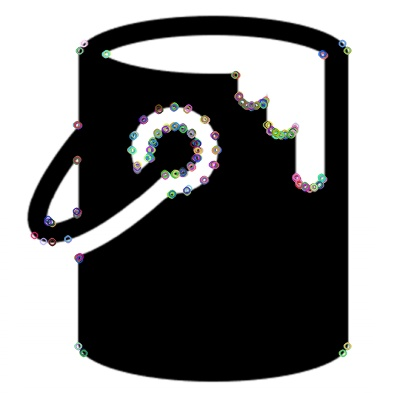
\includegraphics[width=1.0\textwidth]{img/piktogrammerkennung/orb_kp1.jpg}
  \caption{Extrahierte Merkmale mit ORB vom Template}
  \label{fig:orb-kp1}
  \end{minipage} 
  \hfill
  \begin{minipage}[t]{0.45\linewidth}
  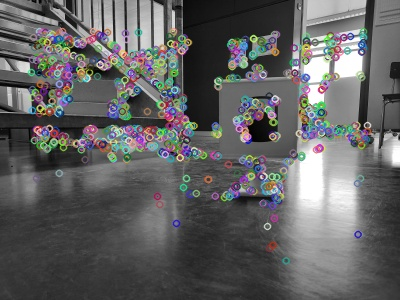
\includegraphics[width=1.0\textwidth]{img/piktogrammerkennung/orb_kp2.jpg}
  \caption{Extrahierte Merkmale mit ORB vom Inputbild}
  \label{fig:orb-kp2}
  \end{minipage}
\end{figure}

\begin{figure}[H]
  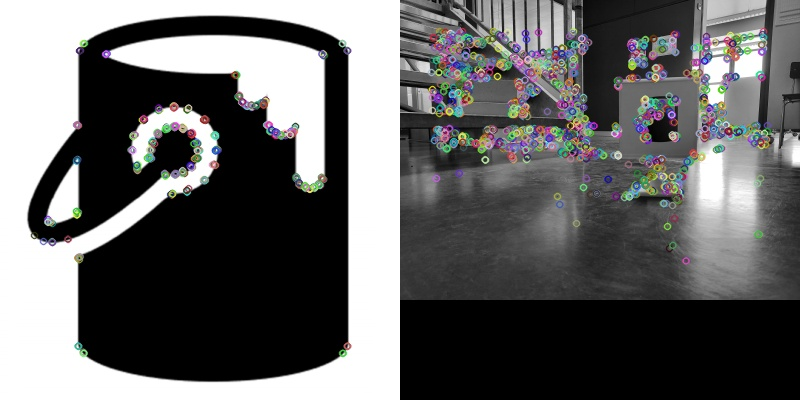
\includegraphics[width=0.95\textwidth]{img/piktogrammerkennung/orb_matches.jpg}
  \centering
  \caption{Matches der ORB Merkmale mit einem Matchverhältniss von 0.75}
  \label{fig:orb-matches-0.75}
\end{figure}

\begin{figure}[H]
  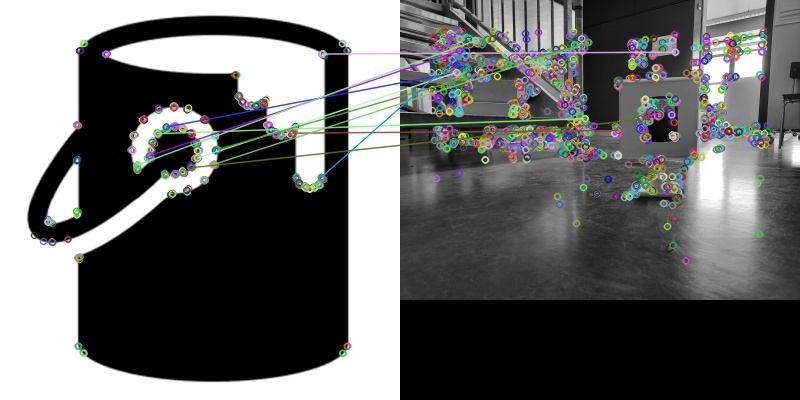
\includegraphics[width=0.95\textwidth]{img/piktogrammerkennung/orb_matches_0.85.jpg}
  \centering
  \caption{Matches der ORB Merkmale mit einem Matchverhältniss von 0.85}
  \label{fig:orb-matches-0.85}
\end{figure}

Matching Results\\
*******************************\\
\# Keypoints 1:                           388\\
\# Keypoints 2:                           1903\\
\# Matches:                               388\\
\# Good Matches:                          0\\

\textbf{SIFT}\\

\begin{figure}[H]
  \centering
  \begin{minipage}[t]{0.45\linewidth}
  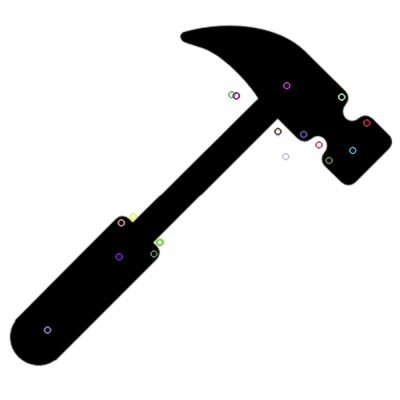
\includegraphics[width=1.0\textwidth]{img/piktogrammerkennung/sift_kp1.jpg}
  \caption{Extrahierte Merkmale mit SIFT vom Template}
  \label{fig:sift-kp1}
  \end{minipage} 
  \hfill
  \begin{minipage}[t]{0.45\linewidth}
  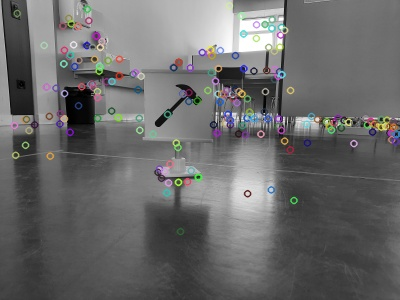
\includegraphics[width=1.0\textwidth]{img/piktogrammerkennung/sift_kp2.jpg}
  \caption{Extrahierte Merkmale mit SIFT vom Inputbild}
  \label{fig:sift-kp2}
  \end{minipage}
\end{figure}

\begin{figure}[H]
  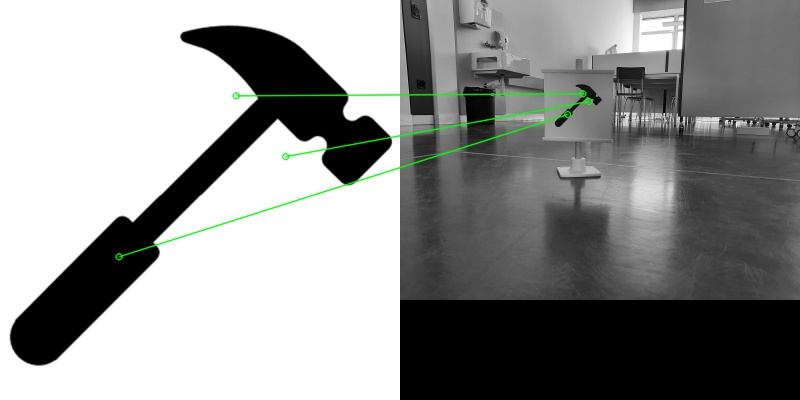
\includegraphics[width=0.95\textwidth]{img/piktogrammerkennung/sift_matches.jpg}
  \centering
  \caption{Matches der SIFT Merkmale mit einem Matchverhältniss von 0.7}
  \label{fig:orb-matches-0.75}
\end{figure}

Matching Results \\
*******************************\\
\# Keypoints 1:                           31\\
\# Keypoints 2:                           233\\
\# Matches:                               31\\
\# Good Matches:                          3\\

\subsubsection{ROI Eingrenzung mittels Histogramm Backprojection}
Bei der Histogramm Backprojection wird ganz grob gesagt, ein Bild erzeugt, bei welchem jedes Pixel die Wahrscheinlichkeit angibt, dass es zum vorgegebenen Template gehört. Ist es zu 100\% wahrscheinlich, dass das Pixel im Inputbild zu einem vorgegebenen Template gehört, wird erhält dies z.B. den Wert 255. Desto weniger gross die Chance ist, desto kleiner wird der Graustufenwert des Pixels.

Diese resultierende Wahrscheinlichkeitsmatrix kann man mithilfe von Thresholding zu einer Maske machen und mit dem Inputbild Multiplizieren oder auch bitweise Und-Verknüpfen. Dann erhält man nur die Stellen des Inputbildes, welche zu einer gewisse Wahrscheinlichkeit (welche beim Thresholding festgelegt wird) zum Template gehören. 

Das Ziel war es also, ahnahnd dieser Maske herauszufinden, auf welche Stelle im Inputbild gezoomt werden soll. So wird verhindert, dass man aus versehen die Stelle welche das Piktogramm beinhaltet wegschneidet.

Auf dem Bild \ref{fig:backprojection-hammer} sind die drei oben beschriebenen Schritte visualisiert. Ganz links ist das Inputbild zu sehen, in der Mitte die Maske welche sich aus der Wahrscheinlichkeitsmatrix ergeben haben. Ganz rechts ist das Resultat aus der Multiplikation von der Maske mit dem Inputbild zu sehen. Als Template wurde das Piktogramm auf folgender Abbildung \ref{fig:sift-kp1} verwendet. Bereits in der Maske aber vorallem auch im Bild ganz rechts ist zu sehen, dass das Piktogramm nicht erkannt wurde. 

\begin{figure}[H]
  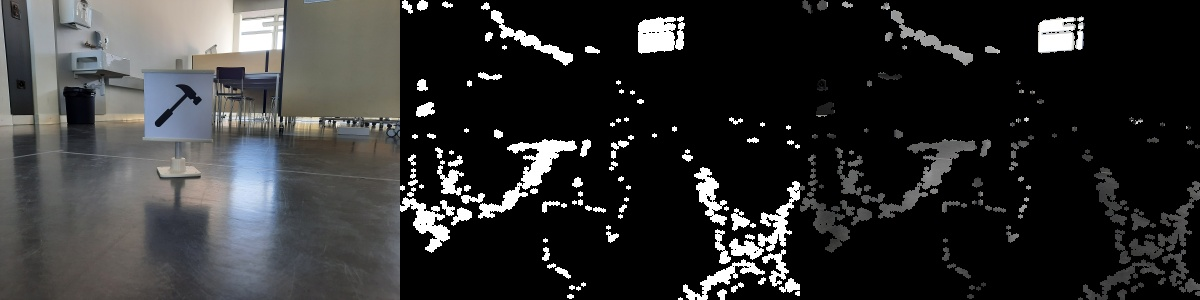
\includegraphics[width=1\textwidth]{img/piktogrammerkennung/hammer_backprojection.jpg}
  \centering
  \caption{Histogramm Backprojection vom Hammer Piktogramm}
  \label{fig:backprojection-hammer}
\end{figure}

Da der selbe Programmcode auf einem anderen Bild viel bessere Resultate erzielte, wurde dieser Ansatz verworfen. Das Bild \ref{fig:backprojection-hand} zeigt, dass der grüne Hintergrund ziemlich gut von den Händen differenziert werden konnten. Ein Grund für die schlechten Ergebnisse mit dem Piktogramm als Template kann sein, dass diese lediglich schwarze und weisse Pixel beinhalten und der Hintergrund des Inputbildes ebenfalls wenig unterschiedliche Farben enthält. Der Algorithmus für die Histogramm Backprojection arbeitet jedoch mit dem HSV-Wert. Somit ist es möglich, dass die HSV-Werte zu wenig grosse Unterschiede aufweisen, als dass diese ohne aufwändiges Finetuneing der Hyperparameter deutlich unterschieden werden können. Wenn man jedoch ein grünes Pixel (HSV: 120) von einem Roten Pixel (HSV: 0) unterscheiden muss, ist dies einfacher, da die Differenz zwischen den HSV-Werten viel deutlicher ist. 

\begin{figure}[H]
  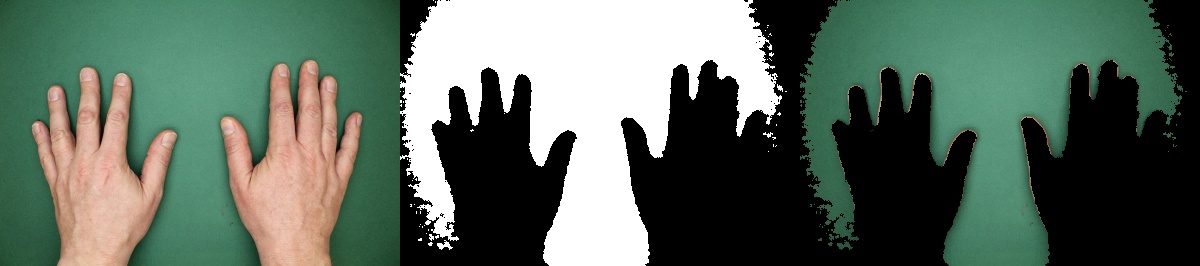
\includegraphics[width=1\textwidth]{img/piktogrammerkennung/hand_backprojection.jpg}
  \centering
  \caption{Histogramm Backprojection vom gut geeignetem Bild}
  \label{fig:backprojection-hand}
\end{figure}


\subsection{ROI Eingrenzung mittels Konturenerkennung}
Um die Genauigkeit des Feature Matching zu erhöhen, wurde eine Idee welche in PREN1 entstanden ist umgesetzt. Das Bild soll auf rechteckige Konturen abgesucht werden. Dabei werden die gefundenen Konturen nach ihrer Fläche sortiert. Man geht dann davon aus, dass es sich beim Rechteck mit der grössten Fläche um das Piktogramm handelt. 

In Abbildung \ref{fig:contour-hammer} ist zu sehen, dass der Algorithmus keine rechteckigen Konturen auf dem Bild mit dem Hammerpiktogramm erkennen konnte. Das Problem ist in Bild \ref{fig:edge-hammer} zu sehen. Die Kanten des Piktogramms werden nicht richtig erkannt. Dies könnte daran liegen, dass die Halterung ebenfalls Weiss ist. Was einen sehr geringen Kontrast zur folge hat und dieser Geringe Kontrast liefert nur sehr flache Gradienten, welche schlussendlich in keiner oder nur einer löchrigen Kante resultieren. Auch durch Tuneing der Parameter der Kantenerkennung, wurden keine konstant besseren Resultate erzielt.

\begin{figure}[H]
  \centering
  \begin{minipage}[t]{0.45\linewidth}
  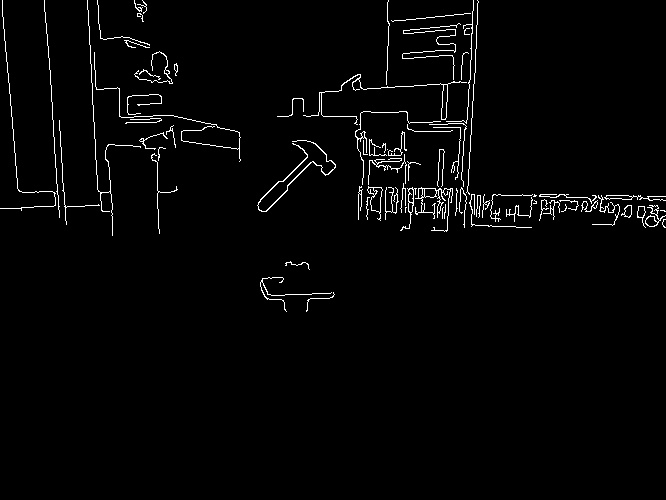
\includegraphics[width=1.0\textwidth]{img/piktogrammerkennung/edge_hammer.jpg}
  \caption{Kantenerkennung des Hammers}
  \label{fig:edge-hammer}
  \end{minipage} 
  \hfill
  \begin{minipage}[t]{0.45\linewidth}
  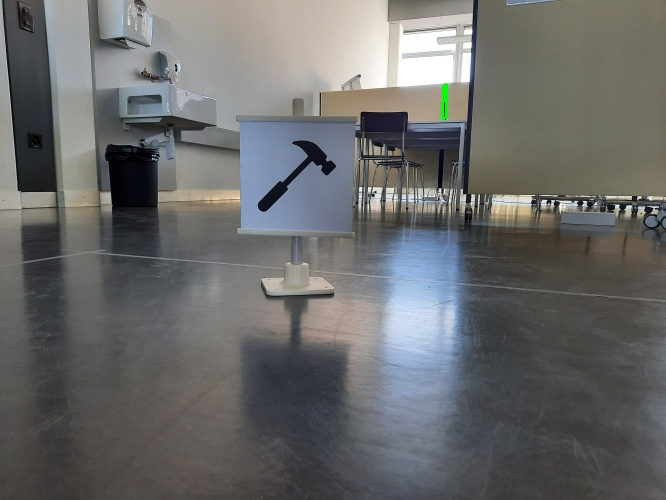
\includegraphics[width=1.0\textwidth]{img/piktogrammerkennung/contours_hammer.jpg}
  \caption{Erkannte Rechteckige Konturen des Hammers}
  \label{fig:contour-hammer}
  \end{minipage}
\end{figure}

Derselbe Algorithmus wurde an einem Beispielbild getestet, welches klare Kanten beinhaltet, welche steile Gradienten zur folge haben. Auf dem nachfolgenden Bild \ref{fig:scanned-doc} sind die Resultate abgebildet. So konnte sichergestellt werden, dass der Algorithmus theoretisch zum gewünschten Ergebnis führt.

\begin{figure}[H]
  \centering
  \begin{minipage}[t]{0.32\linewidth}
  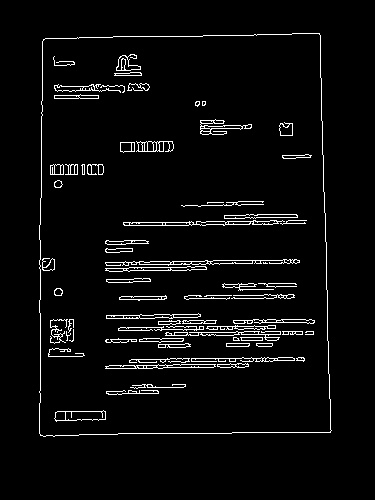
\includegraphics[width=1.0\textwidth]{img/piktogrammerkennung/edge_doc.jpg}
  \caption{Kantenerkennung des optimalen Testbildes}
  \label{fig:edge-doc}
  \end{minipage} 
  \hfill
  \begin{minipage}[t]{0.32\linewidth}
  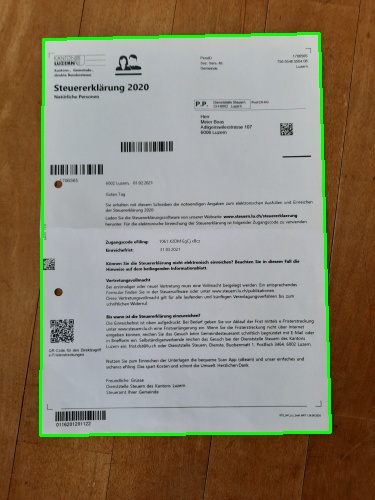
\includegraphics[width=1.0\textwidth]{img/piktogrammerkennung/contours_doc.jpg}
  \caption{Erkannte Rechteckige Konturen des optimalen Testbildes}
  \label{fig:contour-doc}
  \end{minipage}
  \hfill
  \begin{minipage}[t]{0.32\linewidth}
  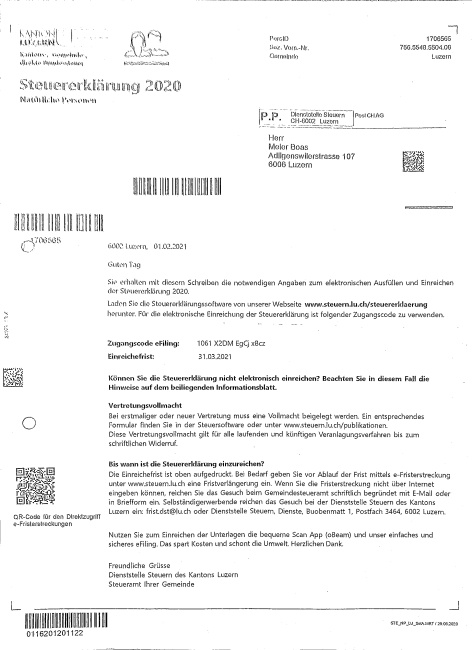
\includegraphics[width=1.0\textwidth]{img/piktogrammerkennung/scanned_doc.jpg}
  \caption{ROI Eingrenzung des optimalen Testbildes}
  \label{fig:scanned-doc}
  \end{minipage}
\end{figure}

\subsubsection{Bild für Detektion in Teilbilder aufteilen}
\label{sec:detektion-auf-teilbildern}
Da man davon ausgegangen ist, das viel Hintergrundfläche einen negativen Einfluss auf die Matchergebnisse hat, war die Idee, das Bild in mehere Teilbilder aufzuteilen. Auf den einzelnen Teilbildern werden dann die Keypunkte extrahiert. Diese Keypunkte werden dann für die Deskription und das Matching auf das gesamte Bild abgetragen.

\begin{figure}[H]
  \centering
  \begin{minipage}[t]{0.22\linewidth}
  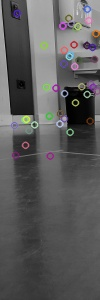
\includegraphics[width=1.0\textwidth]{img/piktogrammerkennung/slice0_kp2.jpg}
  \caption{Extrahierte Merkmale mit SIFT von Slice 0}
  \label{fig:slice0-kp2}
  \end{minipage} 
  \hfill
  \begin{minipage}[t]{0.22\linewidth}
  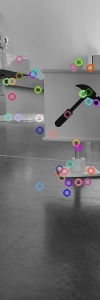
\includegraphics[width=1.0\textwidth]{img/piktogrammerkennung/slice1_kp2.jpg}
  \caption{Extrahierte Merkmale mit SIFT von Slice 1}
  \label{fig:slice1-kp2}
  \end{minipage}
  \hfill
  \begin{minipage}[t]{0.22\linewidth}
  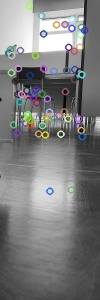
\includegraphics[width=1.0\textwidth]{img/piktogrammerkennung/slice2_kp2.jpg}
  \caption{Extrahierte Merkmale mit SIFT von Slice 2}
  \label{fig:slice2-kp2}
  \end{minipage}
  \hfill
  \begin{minipage}[t]{0.22\linewidth}
  
\includegraphics[width=1.0\textwidth]{img/piktogrammerkennung/slice3_kp2.jpg}
  \caption{Extrahierte Merkmale mit SIFT von Slice 3}
  \label{fig:slice3-kp2}
  \end{minipage}
\end{figure}

\begin{figure}[H]
  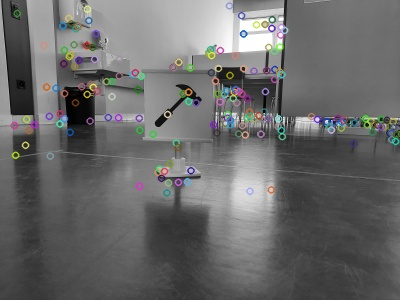
\includegraphics[width=0.95\textwidth]{img/piktogrammerkennung/sift_kp2_from_slice.jpg}
  \centering
  \caption{Matches der ORB Merkmale mit einem Matchverhältniss von 0.85}
  \label{fig:sift-kp2-slice}
\end{figure}

Um die Merkmale auf das uhrsprüngliche Bild zu übertragen, müssen zu deren x-Koordinaten in diesem Fall 100px bzw. 200px bzw. 300px hinzuaddiert werden. Diese 100px ergeben sich daraus, dass das Bild auf 400px Breite skaliert wurde und in vier Streifen von je 100px Breite geschnitten wurde. Hierbei hat sich gezeigt, dass sich die Werte beim anpassen teilweise scheinbar sporadisch leicht ändern. 

Zum Beispiel hat man zu dem Merkmal (6.106937408447266, 81.14856719970703) welches sich im zweiten Slice befindet 100 hinzuaddiert. Nach der Addition scheint der Wert noch zu stimmen: [106.10693740844727, 81.14856719970703]. Nach der Konvertierung in ein Tupel noch immer: (106.10693740844727, 81.14856719970703). Doch sobald die neue Koordinate effektiv dem \texttt{KeyPoint} zugewiesen wurde, stimmt der Wert ab der 6. Nachkommastelle nicht mehr überein: (106.10693359375, 81.14856719970703).

Bei anderen Merkmalen, scheint dies jedoch nicht der Fall zu sein:

(38.83573913574219, 117.7967529296875)\\
(138.8357391357422, 117.7967529296875)\\
(138.8357391357422, 117.7967529296875)\\
(138.8357391357422, 117.7967529296875)\\

Nachfolgend ein Auschnitt des Programmcodes, welcher zu den Keypunkten den entsprechenden Wert hinzuaddiert und von dem auch die obigen Koordinaten ausgegeben wurden:

\begin{minted}{python}
    for kp in kp2[1]:
        nkp = list(kp.pt)
        print(kp.pt)
        nkp[0] = nkp[0] + 100
        print(nkp)
        print(tuple(nkp))
        kp.pt = tuple(nkp)
        print(kp.pt)
    for kp in kp2[2]:
        nkp = list(kp.pt)
        nkp[0] = nkp[0] + 200
        kp.pt = tuple(nkp)
    for kp in kp2[3]:
        nkp = list(kp.pt)
        nkp[0] = nkp[0] + 300
        kp.pt = tuple(nkp)
    kp2 = list(chain.from_iterable(kp2))
\end{minted}

Aufjedenfall, scheint sich diese sporadische Datenkorruption negativ auf die Matchergebnisse auszuwirken. In der Abbildung \ref{fig:sift-matches-slice} ist zu sehen, dass die gematchten Keypunkte nicht mehr zum Piktogramm gehören. 

\begin{figure}[H]
  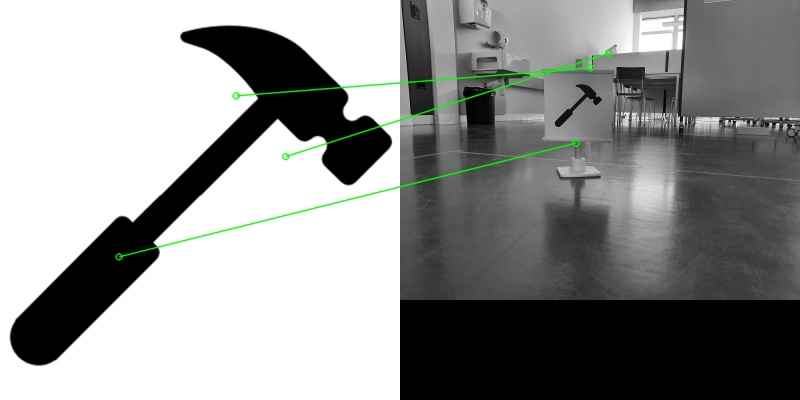
\includegraphics[width=0.95\textwidth]{img/piktogrammerkennung/sift_matches_slice.jpg}
  \centering
  \caption{Matches der SIFT Merkmale aus den verschiedenen Slices mit einem Matchverhältniss von 0.7}
  \label{fig:sift-matches-slice}
\end{figure}

Das oben geschilderte Problem wurde unter anderem nicht mehr weiter untersucht, da beim Auswerten der Anzahl guter Matches aufgefallen ist, dass sich diese in der Anzahl nicht unterscheiden. Ohne Slicing wurde die gleiche Anzahl Matches gefunden wie mit Slicing. Dies löste jedoch den verdacht aus, dass die gefundene Anzahl positiver Matches nicht von der Fläche des unrelevanten Hintergrundes abhängt, sondern von der Skalierung des Bildes. Den bei einem Zoom, bzw. beim wegschneiden des Hintergrundes, wird nicht nur die Hintergrundfläche minimiert, sondern auch automatisch die Skalierung des Piktogramms verändert. Dies aus dem Grund, weil das Inputbild als auch das Template zu beginn des Matchings auf fixe 400 px breite skaliert wird.

Matching Results\\
*******************************\\
\# Keypoints 1:                           31\\
\# Keypoints 2:                           218\\
\# Matches:                               31\\
\# Good Matches:                          3\\

\subsubsection{Skalierung}
Wie bereits am Ende des Kapitels \ref{sec:detektion-auf-teilbildern} beschrieben. Kann es sein, dass nicht die Grösse der unrelevanten Hintergrundfläche die positiven Matches negativ beeinflussen, sondern die Skalierung des Piktogramm selber. Da beide Bilder fix auf 400px Breite skaliert werden, ist das Piktogramm im Inputbild oftmals deutlich kleiner als das Piktogramm im Template. 

Im Bild \ref{fig:sift-matches-800} sind die Ergebnisse zu sehen, wenn das Inputbild lediglich auf 800px Breite skaliert wird und nicht mehr auf 400px wie das Template. Wie vermutet liefert SIFT deutlich bessere Ergebnisse, wenn der Skalierungsunterschied vom Template zum Objekt im Inputbild nicht all zu gross ist. Obwohl es sich bei SIFT und ein Scale Invariantes verfahren handelt, was so viel heisst wie, dass sich die Keypunkte und deren Deskriptoren aufgrund von Skalierung nicht verändern, erzielt man bessere Resultate mit einer grösseren Skalierung des zu detektierenden Objektes. Der Grund dafür ist in den Matching Resultaten zu sehen. Bei einer Skalierung von 800 px werden deutlich mehr Keypunte extrahiert, die Chance auf eine grössere Anzahl positiver Matches steigt also logischerweise an.

\begin{figure}[H]
  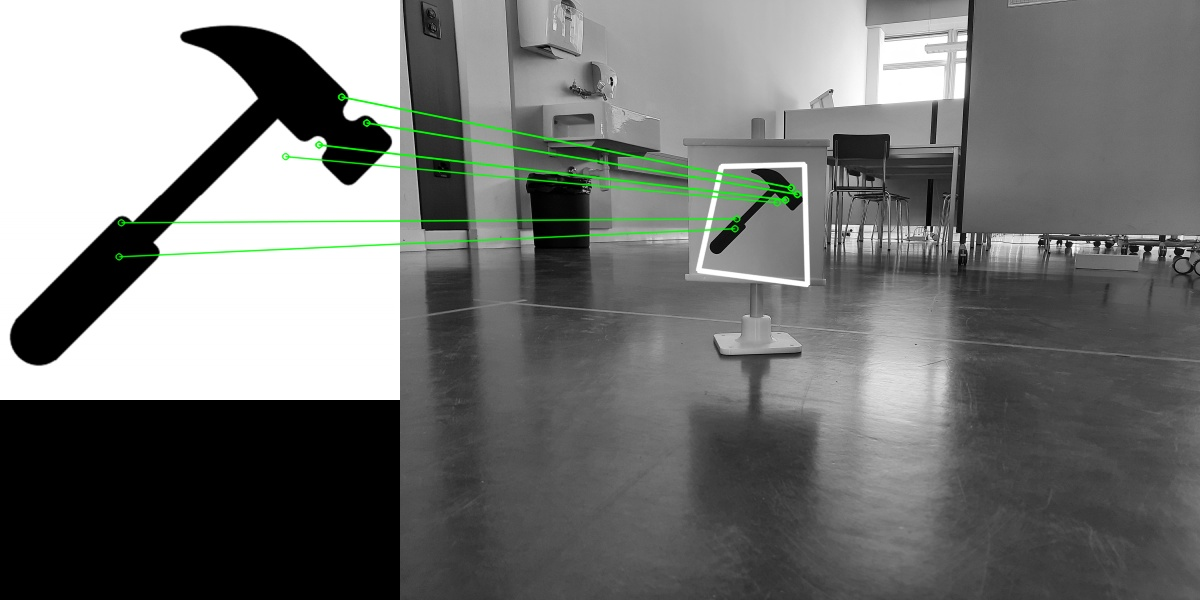
\includegraphics[width=0.95\textwidth]{img/piktogrammerkennung/sift_matches_800.jpg}
  \centering
  \caption{Matches der SIFT Merkmale bei einer Skalierung des Inputbildes auf 800px}
  \label{fig:sift-matches-800}
\end{figure}

Matching Results\\
*******************************\\
\# Keypoints 1:                           31\\
\# Keypoints 2:                           400\\
\# Matches:                               31\\
\# Good Matches:                          13\\

\subsection{Performance}



